% Source: Code/yolo-ablation-bench/detection_report.tex
% Description: YOLOv8n and YOLOv8s meet 20 FPS threshold; larger models provide more detections but sacrifice real-time performance.

\documentclass[border=4pt]{standalone}
\usepackage[T1]{fontenc}
\usepackage{graphicx}
\usepackage{helvet}
\usepackage{lmodern}
\usepackage{pgfplots}
\usepackage{pgfplotstable}
\usepackage{tikz}
\usepackage[dvipsnames,table]{xcolor}
\pgfplotsset{compat=1.18}

\definecolor{garnet}{HTML}{73000A}
\definecolor{midgray}{gray}{0.35}
\definecolor{lightgray}{gray}{0.8}


\newcommand{\headline}[1]{\textcolor{garnet}{\Large\bfseries #1}}
\newcommand{\subhead}[1]{\textcolor{midgray}{\large #1}}

\begin{document}
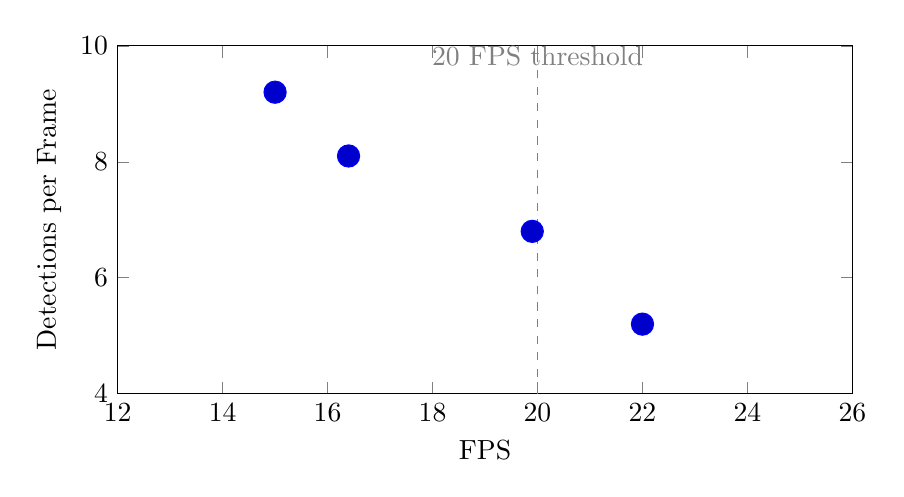
\begin{tikzpicture}
    \begin{axis}[
      width=0.9\textwidth,
      height=6cm,
      xlabel={FPS},
      ylabel={Detections per Frame},
      xmin=12, xmax=26,
      ymin=4, ymax=10,
      nodes near coords,
      every node near coord/.style={anchor=south west, font=\footnotesize},
      scatter/classes={
        nano={mark=square*,garnet},
        small={mark=triangle*,blue!70},
        medium={mark=diamond*,orange!80!black},
        large={mark=o,black!60}
      }
    ]
      % 20 FPS threshold line
      \draw[dashed, gray] (axis cs:20,4) -- (axis cs:20,10);
      \node[gray, anchor=south] at (axis cs:20,9.5) {20 FPS threshold};
      
      % Data points
      \addplot+[scatter, only marks, mark size=4pt] coordinates {
        (22.0, 5.2) [nano]
        (19.9, 6.8) [small]
        (16.4, 8.1) [medium]
        (15.0, 9.2) [large]
      };
    \end{axis}
  \end{tikzpicture}
\end{document}
